\section{SMT and TH RGB LED modules}
\begin{figure}[H]
    \centering
    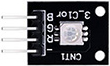
\includegraphics[angle=0, keepaspectratio=true, scale=1, width=200px, height=200px]{images/smd_led.jpg}
    %\caption{Caption}
\end{figure}
\subsection*{Description}
An RGB LED has a pin for each of the three primary colours. The LED module can be controlled by both digital and analog input signals.
\subsection*{Pin mapping}
This pin mapping corresponds to the pins from left to right with the module pins facing towards you.
\begin{table}[H]
    \centering
    \begin{tabular}{|c|c|c|c|c|}
    \hline
    Index &Label &Type &Name &Description\\ \hline
    0 &B &Analog input &A0 &Analog input signal for blue pin \\ \hline
    1 &G &Analog input  &A1 &Analog input signal for green pin \\ \hline
    2 &R &Analog input  &A2 &Analog input signal for red pin \\ \hline
    3 &- &Ground &GND &\\ \hline
    \end{tabular}
    %\caption{Caption}
    %\label{tab:my_label}
\end{table}
\subsection*{Operation}
By applying a PWM signal with varying duty cycle to any of the three pins (A0, A1 and A2) we can control the brightness of each of the three primary colours. Turning multiple colours on at the same time "adds" them together to create other colours.
\subsection*{Code}
Refer to listing \ref{python_rgb}.
%\lstinputlisting[caption=test]{laser.py}